\documentclass[11pt,a4paper,twoside,openright]{memoir}

%%%%%%%%%%%%%%%%%%%%%%%%%%%%%%%%%%%%%%%%%%%%%%%%%%%%%%%
%  In my opinion (DW) there are no fonts available in the standard
%  TeX/LaTeX set that are ideal for this use, unless you go down to 9pt or 
%  8pt for your text face, and this is too small.  If you have Metafont you
%  should consider generating a cmr17 font at a magstep of two (about 25pt)
%  or three (about 30pt), or even more, depending on the point size of your
%  main text.  Why not go the whole hog and design some really fancy 
%  capitals from scratch!
%
%%%%%%%%%%%%%%%%%%%%% BOX ONE %%%%%%%%%%%%%%%%%%%%%%%%%
%\typein[\dropinitialfont]{Font for Dropped initial:} %
%\font\largefont \dropinitialfont                     %
%%%%%%%%%%%%%%%%%%%%%%%%%%%%%%%%%%%%%%%%%%%%%%%%%%%%%%%
%
%%%%%%%%%%%%%%%%%%%%% BOX TWO %%%%%%%%%%%%%%%%%%%%%%%%%
%\font\largefont= cmr10 scaled \magstep5              %
%\font\largefont= cmbx10 scaled \magstep5             %
%\font\largefont= cmbx17 scaled \magstep3             %
\font\largefont= cmr17 scaled \magstep5               %
%%%%%%%%%%%%%%%%%%%%%%%%%%%%%%%%%%%%%%%%%%%%%%%%%%%%%%%

% Copyright Symbole u.�.
\def\TReg{\textsuperscript{\textregistered}}
\def\TCop{\textsuperscript{\textcopyright}}
\def\TTra{\textsuperscript{\texttrademark}}

\def\drop#1#2{{\noindent
    \setbox0\hbox{\largefont #1}\setbox1\hbox{#2}\setbox2\hbox{(}%
    \count0=\ht0\advance\count0 by\dp0\count1\baselineskip
    \advance\count0 by-\ht1\advance\count0by\ht2
    \dimen1=.5ex\advance\count0by\dimen1\divide\count0 by\count1
    \advance\count0 by1\dimen0\wd0
    \advance\dimen0 by.25em\dimen1=\ht0\advance\dimen1 by-\ht1
    \global\hangindent\dimen0\global\hangafter-\count0
    \hskip-\dimen0\setbox0\hbox to\dimen0{\raise-\dimen1\box0\hss}%
    \dp0=0in\ht0=0in\box0}#2}

% end of new \drop command
%%%%%%%%%%%%%%%%%%%%%%%%%%%%%%%%%%%%%%%%%%%%%%%%%%%%%%%

%%%%%%%%%%%%%%%%%%%%%%%%%%%%%%%%%%%%%%%%%%%%%%%%%%%%%%%
% new \versal command
\newcommand{\versal}[1]{{\noindent
    \setbox0\hbox{\largefont #1}%
    \count0=\ht0                   % height of versal
    \count1=\baselineskip          % baselineskip
    \divide\count0 by \count1      % versal height/baselineskip
    \dimen1 = \count0\baselineskip % distance to drop versal
    \advance\count0 by 1\relax     % no of indented lines
    \dimen0=\wd0                   % width of versal
    \global\hangindent\dimen0      % set indentation distance
    \global\hangafter-\count0      % set no of indented lines
    \hskip-\dimen0\setbox0\hbox to\dimen0{\raise-\dimen1\box0\hss}%
    \dp0=0in\ht0=0in\box0}}
% end of new \versal command
%%%%%%%%%%%%%%%%%%%%%%%%%%%%%%%%%%%%%%%%%%%%%%%


%%%%%%%%%%%%%%%%%%%%%%%%%%%%%%%%%%%%%%%%%%%%%%%
% redefining the textblocksize
%%%%%%%%%%%%%%%%%%%%%%%%%%%%%%%%%%%%%%%%%%%%%%%
\setlrmarginsandblock{1in}{1.5in}{*}
\checkandfixthelayout
%%%%%%%%%%%%%%%%%%%%%%%%%%%%%%%%%%%%%%%%%%%%%%%


\usepackage{graphicx}
\usepackage{latexsym}
\usepackage{epsfig}
\usepackage[figuresright]{rotating}
\usepackage{dsfont}
\usepackage{german}
\usepackage[latin1]{inputenc}
%\usepackage[dvips]{color}
\usepackage{colortbl}
	\definecolor{darkblue}{rgb}{0,0,0.4}
	\definecolor{darkgray}{rgb}{0.1,0.1,0.2}
	\definecolor{darkred}{rgb}{0.6,0.0,0.0}
   \definecolor{darkgreen}{rgb}{0.0,0.6,0.0}
   \definecolor{orange}{rgb}{1.0,0.8,0.0}

%---- for algorithms ----
\usepackage[Algorithmus]{algorithm}
\usepackage{algorithmic}

%---- for the index ----
\usepackage{layouts}[2001/04/29]
\makeindex

\usepackage{hyperref}
\usepackage{memhfixc}
\hypersetup{colorlinks=true,linkcolor=darkgray,urlcolor=darkblue,citecolor=darkblue,filecolor=darkgreen}

%---- a second bibliography ----
\usepackage{multibib}
\renewcommand{\refname}{Allgemeine Literaturquellen}

%---- some new math symbols ----
\usepackage{nicefrac} % schr�ge bruchstriche
\usepackage{amssymb}
\newcommand{\Real}{\mathbb R}

%---- memoir package specialties
%\pagestyle{companion}
\pagestyle{Ruled}
\setlength{\epigraphwidth}{7cm}
\setcounter{tocdepth}{3}
\setcounter{secnumdepth}{3}
\maxsecnumdepth{subsection}

% change standard font
%\usepackage{cmbright}
\renewcommand{\rmdefault}{cmss}
\renewcommand{\sfdefault}{cmss}

% set figure resp. table name and number bold
\makeatletter
\renewcommand{\fnum@figure}{\textbf{\figurename~\thefigure}}
\renewcommand{\fnum@table}{\textbf{\tablename~\thetable}}
\makeatother

% setting the authors for a verse
\newcommand{\attrib}[1]{%
	\nopagebreak{\raggedleft\footnotesize #1\par}}

%---- general information ----
\author{ 
	\small{vorgelegt von} \vspace{.5cm} 											\\ 
	\Large{\textbf{Kevin-Horst Bratzke}} 											\\ 
	\small{geb.\ in Leipzig}}
	\title{
			\textbf{\vspace{-2.5cm}
			%--------------------------------------------------------------
			% unter mac os x k�nnen Sie auch ein .png als Bild einbinden...
			%--------------------------------------------------------------
			
\includegraphics[width=16.0cm]{mniLogo.png} \\
			\vspace{3cm} Analyse und Evaluation von unterschiedlichen Schriftsatz-Systemen f�r die Anfertigung von wissenschaftlichen Arbeiten} \\
			\vspace{1cm}
			\normalsize{Studiengang Wirtschaftsmathematik} \vspace{1cm} \\
			\Large{\textbf{Bachelorarbeit}} }
			\date{}


\begin{document}
	%---- the frontmatter ----
	\frontmatter
	
		\begin{titlingpage}
			\begin{center}
				%---- create the title page ----
				\maketitle
				\vspace{-1cm}
				\small{durchgef�hrt am} \\
				\small{Institut f�r Wissenschaftliche Schriften (IWS), Frankfurt}
				\begin{tabular}{ll}
					& \\
					& \\
					& \\
					Referent der Arbeit: & Prof. Dr. Michael Stifel \\
					Korreferent der Arbeit: & Prof. Dr. Gerolamo Cardano \\
					Betreuer am IWS: & Dipl.-Ing. (FH) Seki Takakazu \\
				   & \\
				\end{tabular}

				\vspace{\fill}
				\small{Friedberg, 2014}
			\end{center}
	
		\end{titlingpage}
	
	%---- Widmung ----
	\thispagestyle{empty}
	\begin{flushright}
		\vspace*{\fill}
		\Large{\textsl{\rmfamily{F�r Felix Klein}}}
		\vspace{15cm}
	\end{flushright}

	\cleardoublepage
	\setcounter{page}{1}
	
	%---- Danksagung ----
	\chapter{Danksagung}
Normalerweise haben eine ganze Reihe von Personen mehr oder wenig Anteil am Gelingen der Bachelorarbeit, denen man hier dankt: In der Regel zun�chst den Referenten und Betreuern der Arbeit. Aber nat�rlich auch Personen, Firmen und Institutionen, die die Arbeit tatkr�ftig unterst�tzt haben. Sei es durch die Bereitstellung von spezieller Hard- oder Software oder nur durch ein gewissenhaftes Korrekturlesen.
\\


	%---- Selbstst�ndigkeitserkl�rung ----
	\chapter{Selbstst�ndigkeitserkl�rung}
\label{cha:erklaerung}
%
%
Ich erkl�re, dass ich die eingereichte Bachelorarbeit selbstst�ndig und ohne fremde Hilfe verfasst, andere als die von mir angegebenen Quellen und Hilfsmittel nicht benutzt und die den benutzten Werken w�rtlich oder inhaltlich entnommenen Stellen als solche kenntlich gemacht habe. \\
%
\vspace{.2cm} \\
\noindent Friedberg, Monat 2014 \\
%
\vspace{2cm} \\
\noindent Kevin-Horst Bratzke \\
%
%
%

	
	\cleardoublepage
	
	%---- table of contents ----
	\tableofcontents
	
	\cleardoublepage
	
	%---- list of figures ----
	\listoffigures
	
	%---- the mainmatter ----
	\mainmatter

		%---- Einf�hrung ----
		%
%%%%%%%%%%%%%%%%%%%%%%%%%%%%%%%%%%%%%%%%%%%%%%%%%%%
%
% E I N L E I T U N G
%
%%%%%%%%%%%%%%%%%%%%%%%%%%%%%%%%%%%%%%%%%%%%%%%%%%%
%
\chapter{Einleitung}
\label{cha:introduction}
%
%
Dieses Vorlagendokument soll das Erstellen der eigenen Bachelorarbeit mit LaTeX erleichtern. Es liefert ein bereits vollst�ndig konfiguriertes Dokument, in dem lediglich der Inhalt ausgetauscht werden muss. Formatierung sind voreingestellt und m�ssen nicht abge�ndert werden. Damit ist es m�glich, sich ohne gr��ere Einarbeitungszeit auf den Inhalt der Arbeit zu konzentrieren. \\
\\
\noindent \textbf{\textcolor{darkred}{Hinweis}}: Dies ist keine Anleitung, wie Sie eine Bachelorarbeit verfassen sollen und wie Sie dem wissenschaftlichen Anspruch des Inhalts gerecht werden. Diese Vorlage ist ein technisches Dokument und zeigt beispielsweise, wie Sie Fu�noten setzen und Literatur referenzieren. Nicht behandelt wird hier die Frage, wann und warum Sie eine Fu�note setzen oder eine Referenz verwenden.
%
%
%%%%%%%%%%%%%%%%%%%%%%%%%%%%%%%%%%%%%%%%%%%%%%%%%%%
%
% A U F B A U 
%
%%%%%%%%%%%%%%%%%%%%%%%%%%%%%%%%%%%%%%%%%%%%%%%%%%%
%
\section{Aufbau des Dokuments}
\label{sec:aufbau}
%
Diese Vorlage verwendet die \textit{memoir}-LaTeX-Klasse von Peter Wilson und erzeugt somit ein Buchdokument, das auch zweiseitig gedruckt werden sollte, da zwischen den Kapiteln Leerseiten erzeugt werden. Einstiegspunkt f�r die Bachelorarbeit ist die Datei \texttt{abschlussarbeit.tex}. Tragen Sie zun�chst den Titel der Arbeit und alle Namen ein. Bei hochschulinternen Bachlorarbeiten fallen die Eintragungen \textit{durchgef�hrt am} und \textit{Betreuer in der Firma} nat�rlich weg. \\

Neben den offensichtlichen Eintragungen f�r das Titelblatt wird in dieser Datei auch die Einteilung der Arbeit in Kapitel und Anh�nge vorgenommen. Verwenden Sie am besten f�r jedes Kapitel einen eigenen Unterordner. In jedem dieser Kapitelordner sollte ein Unterordner names \texttt{images} liegen. Dies erleichtert die Arbeit mit und die Suche nach den entsprechenden Abbildungen (siehe auch Abschnitt \ref{sec:abbildungen}). \\

Daneben werden in dieser Datei auch Zusatzpakete mit dem \texttt{usepackage}-Befehl eingebunden, Farben f�r eine farbliche Darstellung von Text und eventuelle Sonderzeichen wie beispielsweise das \textit{Copyright}-Zeichen \TCop oder das \textit{Trademark}-Zeichen \TTra definiert.
%
%
%%%%%%%%%%%%%%%%%%%%%%%%%%%%%%%%%%%%%%%%%%%%%%%%%%%
%
% Abbildungen
%
%%%%%%%%%%%%%%%%%%%%%%%%%%%%%%%%%%%%%%%%%%%%%%%%%%%
%
\section{Abbildungen}
\label{sec:abbildungen}
%
Bilder sollten im \texttt{.eps}-Format (Encapsulated PostScript) eingebunden werden. Wandeln Sie daher eine Grafik, die als \texttt{.jpg}, \texttt{.png} oder in einem anderen Dateiformat vorliegt, vor der Verwendung in Ihrer Bachelorarbeit entsprechend um. Alle g�ngigen Bildbearbeitungsprogramme wie beispielsweise Adobe Photoshop \footnote{http://www.adobe.com/de/products/photoshop/family/} oder Gimp \footnote{http://www.gimp.org/} sind in der Lage, Bilder ins \texttt{EPS}-Format zu exportieren.
%
\begin{figure}
  \centering
   {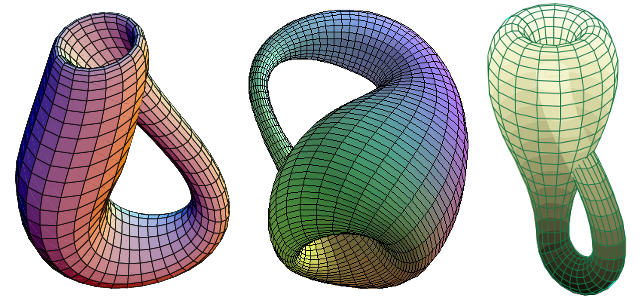
\epsfig{file = intro/images/klein_bottle.png, width=11.0cm}}
  \caption[Kleinsche Flasche]{Drei Versionen der Kleinschen Flasche. Die Objekte sind mit Mathematica (links, Quelle gemeinfrei), Maple (mitte, Quelle: T. Hall) und GnuPlot (rechts, Quelle: O. Alexandrov)	erstellt.}
  \label{fig:klein_bottle}
\end{figure}
%
Wenn Sie auf Abbildungen im Text verweisen wollen, verwenden Sie die \texttt{ref}-Marke: Die \textit{Kleinsche Flasche} \cite{schrijver89} (siehe Abbildung \ref{fig:klein_bottle}) ist ein geometrisches Objekt, das nur eine einzige Seite besitzt. Man kann also nicht zwischen \textit{innen} und \textit{au�en} unterscheiden. Beschriften Sie die Abbildungen ausf�hrlich. Verwenden Sie die beiden Textoptionen in der \texttt{caption}-Marke, um auch eine kurze Beschreibung f�r das Abbildungsverzeichnis zu erzeugen. \\
%
Vergessen Sie bitte nicht, die Eigent�mer eines Bildes zu nennen, wenn Sie ein Bild nicht selbst erstellt haben. \\
%
%
%%%%%%%%%%%%%%%%%%%%%%%%%%%%%%%%%%%%%%%%%%%%%%%%%%%
%
%  L I T E R A T U R V E R W E I S E
%
%%%%%%%%%%%%%%%%%%%%%%%%%%%%%%%%%%%%%%%%%%%%%%%%%%%
%
\section{Literaturverweise}
\label{sec:verweise}
%
Verweise auf Literatur, die Sie in der Ihrer Bachelorarbeit verwenden, sollten in der Datei \texttt{abschlussarbeit.bib} eingetragen werden. In dieser Datei k�nnen durchaus mehr Eintr�ge enthalten sein, als Sie in Ihrer Arbeit als Referenzen verwenden. LaTeX wird nur auch tats�chlich referenzierte Literatur in das Verzeichnis am Ende der Arbeit aufnehmen. Die freie Software LEd (siehe Kapitel \ref{cha:umgebung}) ist in der Lage, Vorlagen f�r die unterschiedlichsten Arten von Literatur aufzunehmen, wie beispielsweise B�cher, Artikel in Zeitschriften oder wissenschaftliche Ver�ffentlichungen in den \textit{Proceedings} von Konferenzen. Denken Sie bitte bei Ihrer Recherchearbeit daran, dass Sie von Rechnern der Hochschule aus freien Zugang zu einer Vielzahl von Online-Bibliotheken wie IEEE\footnote{http://ieeexplore.ieee.org/} und ACM\footnote{http://portal.acm.org/} haben.
%
%
%%%%%%%%%%%%%%%%%%%%%%%%%%%%%%%%%%%%%%%%%%%%%%%%%%%
%
%   F O R M E L N   U N D   T A B E L L E N
%
%%%%%%%%%%%%%%%%%%%%%%%%%%%%%%%%%%%%%%%%%%%%%%%%%%%
%
\section{Verwendung von Formeln und Tabellen}
\label{sec:formeln}
%
W�hrend Tabellen leider schnell un�bersichtlich werden k�nnen, spielt LaTeX bei Formeln sein volles Potential aus. Kein anderes Textsatzsystem erzeugt so schnell und einfach sch�ne Formeln. Im folgenden Abschnitt werden einige Textpassagen vorgestellt, die typische Formeln verwenden. Ein Blick an die entsprechenden Zeilen in der LaTeX-Datei zeigt Ihnen, wie diese Formeln entstehen.\\
\\
Formeln k�nnen direkt in den Text integriert werden: $x_i=x_{x-1} + x_{i-2}$ ist beispielsweise die Rechenvorschrift f�r die Fibonacci-Folge \cite{conway96}. \\
\\
``...Das Kameramodell basiert auf dem Prinzip der Lochkamera und wird f�r eine pr�zise Triangulierung um intrinsische Parameter wie etwa der Linsenverzeichnung erweitert: \\

\noindent \textbf{\textcolor{darkred}{Hinweis}}: Das $\Real$-Zeichen und die dunkelrote Textfarbe sind im Hauptdokument \texttt{abschlussarbeit.tex} definiert.
\begin{tabbing}
Platzhalter links \quad \= Platzhalter Mitte \quad \= Platzhalter rechts \kill
$T \in \Real^3$  \> der Brennpunkt und Ursprung des Kamerakoordinatensystems \\
                 \> im Weltkoordinatensystem und                             \\
$R \in SO_3$     \> die Rotation der Kamera im Weltkoordinatensystem
\end{tabbing}
Als intrinsische Parameter werden
\begin{tabbing}
Platzhalter links \quad \= Platzhalter Mitte \quad \= Platzhalter rechts \kill
$f \in \Real$             \> die Brennweite (fokale L�nge) der Kamera,                                          \\
$P=(u_0,v_0) \in \Real^2$ \> der Hauptpunkt des Bildes (engl.: \textit{principle point}), also der Schnittpunkt \\
                          \> der optischen Achse mit der dazu orthogonal stehenden Bildebene,                   \\
$r_u,r_v \in \Real$       \> Skalierungsfaktoren in x- und y-Richtung auf der Bildebene,                        \\
$s \in \Real$             \> ein Verzerrungsfaktor (engl.: \textit{skew}) der Kameralinse und                   \\
$\kappa \in \Real$        \> die radiale Verzeichnung der Kameralinse
\end{tabbing}
gew�hlt.\\
%
Mit Hilfe der Strahlens�tze ist die Projektion durch $(\nicefrac{-f \cdot x_c}{z_c}, \nicefrac{-f \cdot y_c}{z_c})^T$ zu berechnen. Die restlichen intrinsischen Kameraparameter lassen sich in der Kamerakalibrierungsmatrix $K$ mit
\begin{equation}
\label{eqn:K}
\left(\begin{array}{ccc}r_u&s&u_0\\0&r_v&v_0\\0&0&1 \end{array}\right) \cdot 
\left(\begin{array}{c}\nicefrac{-f \cdot x_c}{z_c}\\\nicefrac{-f \cdot y_c}{z_c}\\1\end{array}\right) = 
\underbrace{\left(\begin{array}{ccc}-f \cdot r_u&-f \cdot s&u_0\\0&-f \cdot r_v&v_0\\0&0&1 \end{array}\right)}_{=K} \cdot 
\left(\begin{array}{c}\nicefrac{x_c}{z_c}\\\nicefrac{y_c}{z_c}\\1\end{array}\right)
\end{equation}
zusammenfassen. Diese Matrix wird so genannt, da alle intrinsischen Konstanten der Kalibrierung in einer einzigen Matrix enthalten sind. \\
%
Die Summe der $m$ Abst�nde zwischen Originalpunkt und projiziertem Punkt in der Bildebene der zweiten Kamera wird mit
\begin{equation}
\sum_{i=1..m}r_i = \sum_{i=1..m} \Vert\tilde U^2_i - U^2_i \Vert
\end{equation}
minimiert.''\\
%

Nun ein Beispiel, bei dem zwei Formeln in einer Zeile stehen, das verbindende \textit{UND} aber nicht als Formeltext, sondern als normaler Flusstext erscheint: ``...Als erster Schritt der Rekonstruktion werden beide 2D-Punkte um einen Tiefenwert erweitert, um 3D-Koordinaten zu erhalten:''
%
\begin{equation}
\bar{U}^1=\left(\begin{array}{c}U^1\\-f_1\end{array}\right) \in \Real^3 \quad \mbox{und} \quad
\bar{U}^2=\left(\begin{array}{c}U^2\\-f_2\end{array}\right) \in \Real^3
\end{equation}
%

Am Ende dieses Abschnitts noch ein Beispiel f�r eine Tabelle:\\
``Die folgende Tabelle \ref{tab:vergleich} stellt die vier Verfahren in einem direkten Vergleich in Bezug auf die drei Parameter gegen�ber:''
%
%
%  T A B L E   V E R G L E I C H
%
\begin{table}[H]
\centering{
\caption{Vergleich verschiedener Algorithmen.}
\label{tab:vergleich}
\begin{tabular}{p{2.5cm}p{2.5cm}p{2.5cm}p{2.5cm}p{2.5cm}}
  \hline \addlinespace
   & \textbf{Verfahren 1} & \textbf{Verfahren 2} & \textbf{Verfahren 3} & \textbf{Verfahren 4} \\
  \addlinespace \hline \addlinespace
  \textbf{Lexikoneintrag} & nein & ja & ja & nein \\
  \addlinespace \hline \addlinespace
  \textbf{Trainings\-aufwand} & keiner & keiner & 2 min bei \newline Optimierung\textsuperscript{1} & keiner \\
  \addlinespace \hline \addlinespace
  \textbf{Ergebnis} & 22 sec & 32 sec & 30 sec & 13 sec \\
  \addlinespace \hline
\end{tabular}}
\end{table}
%\vspace{1mm}
\noindent \textsuperscript{1} Anmerkungen zu Tabelleneintr�gen k�nnen am Ende der Tabelle erkl�rt werden. \vspace{2mm} \\
%
Lorem ipsum dolor sit amet, consectetur adipisici elit, sed eiusmod tempor incidunt ut labore et dolore magna aliqua. Ut enim ad minim veniam, quis nostrud exercitation ullamco laboris nisi ut aliquid ex ea commodi consequat. Quis aute iure reprehenderit in voluptate velit esse cillum dolore eu fugiat nulla pariatur. Excepteur sint obcaecat cupiditat non proident, sunt in culpa qui officia deserunt mollit anim id est laborum. \\


		%---- Kapitel MikTeX ----
		%
%%%%%%%%%%%%%%%%%%%%%%%%%%%%%%%%%%%%%%%%%%%%%%%%%%%
%
%  E N T W I C K L U N G S U M G E B U N G
%
%%%%%%%%%%%%%%%%%%%%%%%%%%%%%%%%%%%%%%%%%%%%%%%%%%%
\chapter{Entwicklungsumgebung}
\label{cha:umgebung}
%
%
Als Entwicklungsumgebung f�r die Erstellung und Bearbeitung von Latex-Dokumenten unter Windows eignet sich am besten die Kombination aus MiKTeX\footnote{www.miktex.org} und TeXstudio\footnote{texstudio.sourceforge.net/}. Auf heise.de\footnote{www.heise.de/software} kann man auch drekt das TeXstudio als Portable-Version herunterladen, die nicht einmal installiert werden muss und auf jedem USB-Stick Platz findet.\\

Laden und installieren Sie zun�chst MiKTeX, dann installieren oder �ffnen Sie das TeXstudio. Laden Sie die Haupt-.tex-Datei der Abschlussarbeit. Auf der linken Seite sollten nun auch alle Einzelkapitel, Anh�nge und das Glossar angezeigt werden. Durch dr�cken des gr�nen Doppelpfleils in der Icon-Leiste wird das fertige .pdf erstellt und direkt im Studio angezeigt. Au�erdem liegt das fertige .pdf nat�rlich auch im Projektordner.\\

Zum Bearbeiten eines Kapitels Ihrer Abschlussarbeit dr�cken Sie einfach im linken Struktur-Fenster auf das entsprechende Kapitel und editieren Sie den Inhalt.\\ 


	%---- Beginn Anhang ----
	\appendix	% resets numbering to alphabetic style
	%
%
\chapter{Lorem Ipsum}
%
%
Lorem ipsum dolor sit amet, consectetur adipisici elit, sed eiusmod tempor incidunt ut labore et dolore magna aliqua. Ut enim ad minim veniam, quis nostrud exercitation ullamco laboris nisi ut aliquid ex ea commodi consequat. Quis aute iure reprehenderit in voluptate velit esse cillum dolore eu fugiat nulla pariatur. Excepteur sint obcaecat cupiditat non proident, sunt in culpa qui officia deserunt mollit anim id est laborum.
\\
Duis autem vel eum iriure dolor in hendrerit in vulputate velit esse molestie consequat, vel illum dolore eu feugiat nulla facilisis at vero eros et accumsan et iusto odio dignissim qui blandit praesent luptatum zzril delenit augue duis dolore te feugait nulla facilisi. Lorem ipsum dolor sit amet, consectetuer adipiscing elit, sed diam nonummy nibh euismod tincidunt ut laoreet dolore magna aliquam erat volutpat.
\\
Ut wisi enim ad minim veniam, quis nostrud exerci tation ullamcorper suscipit lobortis nisl ut aliquip ex ea commodo consequat. Duis autem vel eum iriure dolor in hendrerit in vulputate velit esse molestie consequat, vel illum dolore eu feugiat nulla facilisis at vero eros et accumsan et iusto odio dignissim qui blandit praesent luptatum zzril delenit augue duis dolore te feugait nulla facilisi.
\\
Nam liber tempor cum soluta nobis eleifend option congue nihil imperdiet doming id quod mazim placerat facer possim assum. Lorem ipsum dolor sit amet, consectetuer adipiscing elit, sed diam nonummy nibh euismod tincidunt ut laoreet dolore magna aliquam erat volutpat. Ut wisi enim ad minim veniam, quis nostrud exerci tation ullamcorper suscipit lobortis nisl ut aliquip ex ea commodo consequat.
\\
Duis autem vel eum iriure dolor in hendrerit in vulputate velit esse molestie consequat, vel illum dolore eu feugiat nulla facilisis.
\\
At vero eos et accusam et justo duo dolores et ea rebum. Stet clita kasd gubergren, no sea takimata sanctus est Lorem ipsum dolor sit amet. Lorem ipsum dolor sit amet, consetetur sadipscing elitr, sed diam nonumy eirmod tempor invidunt ut labore et dolore magna aliquyam erat, sed diam voluptua. At vero eos et accusam et justo duo dolores et ea rebum. Stet clita kasd gubergren, no sea takimata sanctus est Lorem ipsum dolor sit amet. Lorem ipsum dolor sit amet, consetetur sadipscing elitr, At accusam aliquyam diam diam dolore dolores duo eirmod eos erat, et nonumy sed tempor et et invidunt justo labore Stet clita ea et gubergren, kasd magna no rebum. sanctus sea sed takimata ut vero voluptua. est Lorem ipsum dolor sit amet. Lorem ipsum dolor sit amet, consetetur sadipscing elitr, sed diam nonumy eirmod tempor invidunt ut labore et dolore magna aliquyam erat.
\\
Consetetur sadipscing elitr, sed diam nonumy eirmod tempor invidunt ut labore et dolore magna aliquyam erat, sed diam voluptua. At vero eos et accusam et justo duo dolores et ea rebum. Stet clita kasd gubergren, no sea takimata sanctus est Lorem ipsum dolor sit amet. Lorem ipsum dolor sit amet, consetetur sadipscing elitr, sed diam nonumy eirmod tempor invidunt ut labore et dolore magna aliquyam erat, sed diam voluptua. At vero eos et accusam et justo duo dolores et ea rebum. Stet clita kasd gubergren, no sea takimata sanctus est Lorem ipsum dolor sit amet. Lorem ipsum dolor sit amet, consetetur sadipscing elitr, sed diam nonumy eirmod tempor invidunt ut labore et dolore magna aliquyam erat, sed diam voluptua. At vero eos et accusam et justo duo dolores et ea rebum. Stet clita kasd gubergren, no sea takimata sanctus est Lorem ipsum dolor sit amet.

	%---- Ende Anhang ----

	\cleardoublepage



	% ---- the backmatter ----
	\backmatter
	
		%---- include Glossar ----
		%
%%%%%%%%%%%%%%%%%%%%%%%%%%%%%%%%%%%%%%%%%%%%%%%%%%%
%
% G L O S S A R
%
%%%%%%%%%%%%%%%%%%%%%%%%%%%%%%%%%%%%%%%%%%%%%%%%%%%
\chapter{Glossar}
\label{cha:glossar}


\begin{tabular}{p{3cm} p{12cm}}

LaTeX & Softwarepaket, das die Benutzung des Textsatzprogramms TeX mit Hilfe von Makros vereinfacht.\\
\\
LEd & LaTeX-Editor als freie Software verf�gbar unter: www.latexeditor.org/ \\
\\
\end{tabular}


		%---- Literaturverzeichnis ----
%		\begin{footnotesize}
			\bibliography{abschlussarbeit}
			\bibliographystyle{alphadin}
%		\end{footnotesize}
		
		%---- Own publications again ----
		\cleardoublepage

		%---- Indexverzeichnis ----	
		\cleardoublepage
%		\pagestyle{index}
%		\renewcommand{\chaptermark}[1]{}
		\renewcommand{\preindexhook}{ % Die erste angegebene Seitenzahl ist gew�hnlich, aber nicht immer, die erste Referenz zum entsprechenden Eintrag.
		\vskip\onelineskip}
		\indexintoc
		\printindex
		\cleardoublepage

	
\end{document}
